\section{实验过程}
\subsection{编写词法分析程序}
\subsubsection{lex.l}
\begin{minted}[bgcolor=bg, linenos, breaklines]{c++}
%{
#include <bits/stdc++.h>
#include "y.tab.hh"
extern "C"{
int yywrap(void);
int yylex(void);
}
using namespace std;
%}

digit                           [0-9]
exponent                        ([Ee][+-]?{digit}+)

%%

[-/+*()]                        { yylval.char_value = yytext[0];     return yytext[0]; }
0|([1-9]{digit}*?)              { yylval.double_value = atoi(yytext); return CONSTANT; }
{digit}+{exponent}?             { yylval.double_value = atof(yytext); return CONSTANT; }
{digit}*"."{digit}+{exponent}?  { yylval.double_value = atof(yytext); return CONSTANT; }
{digit}+"."{digit}*{exponent}?? { yylval.double_value = atof(yytext); return CONSTANT; }

%%

int yywrap(void) {
  return 1;
}
\end{minted}
使用lex识别运算符和数字

\subsubsection{lex.y}
\begin{minted}[bgcolor=bg, linenos, breaklines]{c++}
%union {
  char char_value;
  double double_value;
}

%start E

%token <double_value> CONSTANT
%type <double_value> E T F

%left <char_value> '+' '-' '*' '/'
%token <char_value> '(' ')'
\end{minted}
重写yylval类型并给予所有文法符号定义类型以进行值传递和输出。


\begin{minted}[bgcolor=bg, linenos, breaklines]{c++}
E : E '+' T { $$ = $1 + $3 ;}
  | E '-' T { $$ = $1 - $3 ;}
  | T       { $$ = $1      ;}
  ;

T : T '*' F {$$ = $1 * $3  ;}
  | T '/' F { $$ = $1 / $3 ;}
  | F       { $$ = $1      ;}
  ;

F : '(' E ')' { $$ = $2    ;}
  | CONSTANT  { $$ = $1    ;}
  ;
\end{minted}
声明产生式,并进行数值运算。

\subsubsection{生成词法分析程序}
\begin{minted}[bgcolor=bg, breaklines]{bash}
  flex lex.l ; bison -vd --debug lex.y -o y.tab.cc ; g++ lex.yy.c y.tab.cc -o lex
\end{minted}

\subsubsection{LARA项目簇与DFA}
\begin{minted}[bgcolor=bg]{text}
Grammar

    0 $accept: E $end

    1 E: E '+' T
    2  | E '-' T
    3  | T

    4 T: T '*' F
    5  | T '/' F
    6  | F

    7 F: '(' E ')'
    8  | CONSTANT


Terminals, with rules where they appear

$end (0) 0
'(' (40) 7
')' (41) 7
'*' (42) 4
'+' (43) 1
'-' (45) 2
'/' (47) 5
error (256)
CONSTANT (258) 8


Nonterminals, with rules where they appear

$accept (10)
    on left: 0
E (11)
    on left: 1 2 3, on right: 0 1 2 7
T (12)
    on left: 4 5 6, on right: 1 2 3 4 5
F (13)
    on left: 7 8, on right: 4 5 6


State 0

    0 $accept: . E $end

    CONSTANT  shift, and go to state 1
    '('       shift, and go to state 2

    E  go to state 3
    T  go to state 4
    F  go to state 5


State 1

    8 F: CONSTANT .

    $default  reduce using rule 8 (F)


State 2

    7 F: '(' . E ')'

    CONSTANT  shift, and go to state 1
    '('       shift, and go to state 2

    E  go to state 6
    T  go to state 4
    F  go to state 5


State 3

    0 $accept: E . $end
    1 E: E . '+' T
    2  | E . '-' T

    $end  shift, and go to state 7
    '+'   shift, and go to state 8
    '-'   shift, and go to state 9


State 4

    3 E: T .
    4 T: T . '*' F
    5  | T . '/' F

    '*'  shift, and go to state 10
    '/'  shift, and go to state 11

    $default  reduce using rule 3 (E)


State 5

    6 T: F .

    $default  reduce using rule 6 (T)


State 6

    1 E: E . '+' T
    2  | E . '-' T
    7 F: '(' E . ')'

    '+'  shift, and go to state 8
    '-'  shift, and go to state 9
    ')'  shift, and go to state 12


State 7

    0 $accept: E $end .

    $default  accept


State 8

    1 E: E '+' . T

    CONSTANT  shift, and go to state 1
    '('       shift, and go to state 2

    T  go to state 13
    F  go to state 5


State 9

    2 E: E '-' . T

    CONSTANT  shift, and go to state 1
    '('       shift, and go to state 2

    T  go to state 14
    F  go to state 5


State 10

    4 T: T '*' . F

    CONSTANT  shift, and go to state 1
    '('       shift, and go to state 2

    F  go to state 15


State 11

    5 T: T '/' . F

    CONSTANT  shift, and go to state 1
    '('       shift, and go to state 2

    F  go to state 16


State 12

    7 F: '(' E ')' .

    $default  reduce using rule 7 (F)


State 13

    1 E: E '+' T .
    4 T: T . '*' F
    5  | T . '/' F

    '*'  shift, and go to state 10
    '/'  shift, and go to state 11

    $default  reduce using rule 1 (E)


State 14

    2 E: E '-' T .
    4 T: T . '*' F
    5  | T . '/' F

    '*'  shift, and go to state 10
    '/'  shift, and go to state 11

    $default  reduce using rule 2 (E)


State 15

    4 T: T '*' F .

    $default  reduce using rule 4 (T)


State 16

    5 T: T '/' F .

    $default  reduce using rule 5 (T)
\end{minted}

\subsubsection{分析过程}
\subsubsubsection{测试用例}
\begin{lstlisting}
(3+5/2)*(2.4/3)-(1-2)
\end{lstlisting}
\subsubsubsection{分析过程}
\begin{minted}[bgcolor=bg, linenos, breaklines]{text}
Starting parse
Entering state 0
Reading a token: Next token is token '(' ('(')
Shifting token '(' ('(')
Entering state 2
Reading a token: Next token is token CONSTANT (3)
Shifting token CONSTANT (3)
Entering state 1
Reducing stack by rule 8 (line 55):
   $1 = token CONSTANT (3)
-> $$ = nterm F (3)
Stack now 0 2
Entering state 5
Reducing stack by rule 6 (line 51):
   $1 = nterm F (3)
-> $$ = nterm T (3)
Stack now 0 2
Entering state 4
Reading a token: Next token is token '+' ('+')
Reducing stack by rule 3 (line 46):
   $1 = nterm T (3)
-> $$ = nterm E (3)
Stack now 0 2
Entering state 6
Next token is token '+' ('+')
Shifting token '+' ('+')
Entering state 8
Reading a token: Next token is token CONSTANT (5)
Shifting token CONSTANT (5)
Entering state 1
Reducing stack by rule 8 (line 55):
   $1 = token CONSTANT (5)
-> $$ = nterm F (5)
Stack now 0 2 6 8
Entering state 5
Reducing stack by rule 6 (line 51):
   $1 = nterm F (5)
-> $$ = nterm T (5)
Stack now 0 2 6 8
Entering state 13
Reading a token: Next token is token '/' ('/')
Shifting token '/' ('/')
Entering state 11
Reading a token: Next token is token CONSTANT (2)
Shifting token CONSTANT (2)
Entering state 1
Reducing stack by rule 8 (line 55):
   $1 = token CONSTANT (2)
-> $$ = nterm F (2)
Stack now 0 2 6 8 13 11
Entering state 16
Reducing stack by rule 5 (line 50):
   $1 = nterm T (5)
   $2 = token '/' ('/')
   $3 = nterm F (2)
-> $$ = nterm T (2.500000)
Stack now 0 2 6 8
Entering state 13
Reading a token: Next token is token ')' (')')
Reducing stack by rule 1 (line 44):
   $1 = nterm E (3)
   $2 = token '+' ('+')
   $3 = nterm T (2.500000)
-> $$ = nterm E (5.500000)
Stack now 0 2
Entering state 6
Next token is token ')' (')')
Shifting token ')' (')')
Entering state 12
Reducing stack by rule 7 (line 54):
   $1 = token '(' ('(')
   $2 = nterm E (5.500000)
   $3 = token ')' (')')
-> $$ = nterm F (5.500000)
Stack now 0
Entering state 5
Reducing stack by rule 6 (line 51):
   $1 = nterm F (5.500000)
-> $$ = nterm T (5.500000)
Stack now 0
Entering state 4
Reading a token: Next token is token '*' ('*')
Shifting token '*' ('*')
Entering state 10
Reading a token: Next token is token '(' ('(')
Shifting token '(' ('(')
Entering state 2
Reading a token: Next token is token CONSTANT (2.400000)
Shifting token CONSTANT (2.400000)
Entering state 1
Reducing stack by rule 8 (line 55):
   $1 = token CONSTANT (2.400000)
-> $$ = nterm F (2.400000)
Stack now 0 4 10 2
Entering state 5
Reducing stack by rule 6 (line 51):
   $1 = nterm F (2.400000)
-> $$ = nterm T (2.400000)
Stack now 0 4 10 2
Entering state 4
Reading a token: Next token is token '/' ('/')
Shifting token '/' ('/')
Entering state 11
Reading a token: Next token is token CONSTANT (3)
Shifting token CONSTANT (3)
Entering state 1
Reducing stack by rule 8 (line 55):
   $1 = token CONSTANT (3)
-> $$ = nterm F (3)
Stack now 0 4 10 2 4 11
Entering state 16
Reducing stack by rule 5 (line 50):
   $1 = nterm T (2.400000)
   $2 = token '/' ('/')
   $3 = nterm F (3)
-> $$ = nterm T (0.800000)
Stack now 0 4 10 2
Entering state 4
Reading a token: Next token is token ')' (')')
Reducing stack by rule 3 (line 46):
   $1 = nterm T (0.800000)
-> $$ = nterm E (0.800000)
Stack now 0 4 10 2
Entering state 6
Next token is token ')' (')')
Shifting token ')' (')')
Entering state 12
Reducing stack by rule 7 (line 54):
   $1 = token '(' ('(')
   $2 = nterm E (0.800000)
   $3 = token ')' (')')
-> $$ = nterm F (0.800000)
Stack now 0 4 10
Entering state 15
Reducing stack by rule 4 (line 49):
   $1 = nterm T (5.500000)
   $2 = token '*' ('*')
   $3 = nterm F (0.800000)
-> $$ = nterm T (4.400000)
Stack now 0
Entering state 4
Reading a token: Next token is token '-' ('-')
Reducing stack by rule 3 (line 46):
   $1 = nterm T (4.400000)
-> $$ = nterm E (4.400000)
Stack now 0
Entering state 3
Next token is token '-' ('-')
Shifting token '-' ('-')
Entering state 9
Reading a token: Next token is token '(' ('(')
Shifting token '(' ('(')
Entering state 2
Reading a token: Next token is token CONSTANT (1)
Shifting token CONSTANT (1)
Entering state 1
Reducing stack by rule 8 (line 55):
   $1 = token CONSTANT (1)
-> $$ = nterm F (1)
Stack now 0 3 9 2
Entering state 5
Reducing stack by rule 6 (line 51):
   $1 = nterm F (1)
-> $$ = nterm T (1)
Stack now 0 3 9 2
Entering state 4
Reading a token: Next token is token '-' ('-')
Reducing stack by rule 3 (line 46):
   $1 = nterm T (1)
-> $$ = nterm E (1)
Stack now 0 3 9 2
Entering state 6
Next token is token '-' ('-')
Shifting token '-' ('-')
Entering state 9
Reading a token: Next token is token CONSTANT (2)
Shifting token CONSTANT (2)
Entering state 1
Reducing stack by rule 8 (line 55):
   $1 = token CONSTANT (2)
-> $$ = nterm F (2)
Stack now 0 3 9 2 6 9
Entering state 5
Reducing stack by rule 6 (line 51):
   $1 = nterm F (2)
-> $$ = nterm T (2)
Stack now 0 3 9 2 6 9
Entering state 14
Reading a token: Next token is token ')' (')')
Reducing stack by rule 2 (line 45):
   $1 = nterm E (1)
   $2 = token '-' ('-')
   $3 = nterm T (2)
-> $$ = nterm E (-1)
Stack now 0 3 9 2
Entering state 6
Next token is token ')' (')')
Shifting token ')' (')')
Entering state 12
Reducing stack by rule 7 (line 54):
   $1 = token '(' ('(')
   $2 = nterm E (-1)
   $3 = token ')' (')')
-> $$ = nterm F (-1)
Stack now 0 3 9
Entering state 5
Reducing stack by rule 6 (line 51):
   $1 = nterm F (-1)
-> $$ = nterm T (-1)
Stack now 0 3 9
Entering state 14
Reading a token:
Now at end of input.
Reducing stack by rule 2 (line 45):
   $1 = nterm E (4.400000)
   $2 = token '-' ('-')
   $3 = nterm T (-1)
-> $$ = nterm E (5.400000)
Stack now 0
Entering state 3
Now at end of input.
Shifting token $end ()
Entering state 7
Stack now 0 3 7
Cleanup: popping token $end ()
Cleanup: popping nterm E (5.400000)
\end{minted}

最后计算得表达式值为5.4与实际吻合极好

\begin{figure}[H]
  \centering
  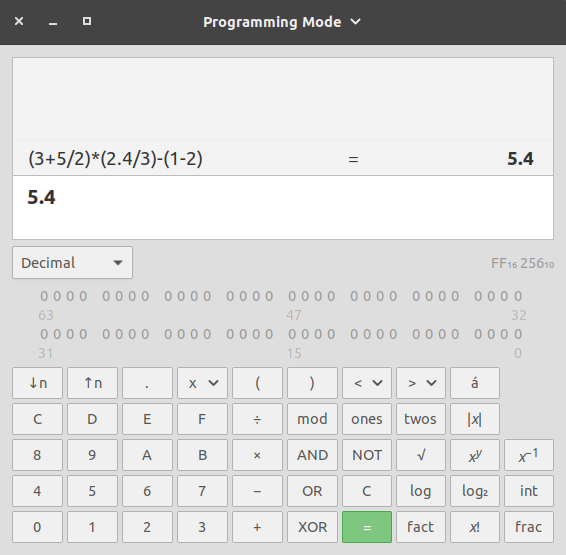
\includegraphics[scale=0.8]{figures/calc.png}
\end{figure}